\documentclass[11pt]{book}

\setcounter{chapter}{16}
\newcommand{\docclass}{CSC 341 (20sp)}
\newcommand{\doctitle}{Mapping Reducibility}
\newcommand{\docauthor}{Peter-Michael Osera}

\usepackage{reading}

\begin{document}

\begin{center}
  \large\textbf{{\doctitle}}
\end{center}

\vspace{2em}

%%%%% Problem-specific Macros %%%%%%%%%%%%%%%%%%%%%%%%%%%%%%%%%%%%%%%%%%%%%%%%%%

\newcommand{\desc}[1]{\ensuremath{\langle #1 \rangle}}
\newcommand{\NP}{\ensuremath{\mathsf{NP}}\xspace}
\newcommand{\prob}[1]{\ensuremath{\mathsf{#1}}\xspace}

%%%%%%%%%%%%%%%%%%%%%%%%%%%%%%%%%%%%%%%%%%%%%%%%%%%%%%%%%%%%%%%%%%%%%%%%%%%%%%%%

\begin{problem}{Graph Reductions}
  Define the following problems:
  \begin{gather*}
    \prob{CLIQUE} = \{ \desc{G, k} \mid \text{ \( G \) has a \( k \)-clique } \} \\
    \prob{COVER}  = \{ \desc{G, k} \mid \text{ \( G \) has a \( k \)-vertex cover } \}
  \end{gather*}
  A \( k \)-clique is a \( k \)-complete subgraph of \( G \).
  A \( k \)-vertex cover is a \( k \)-sized subset of vertices of \( G \) that
  cover (\ie, are \emph{incident} with) all the edges of \( G \).
  Assume that \prob{CLIQUE} is \NP-complete.
  Show that \prob{COVER} is \NP-complete.
\end{problem}

\newpage

\begin{problem}{Card Reductions}
  (Sipser 7.28)
  You are given a box and a collection of cards as indicated in the following figure.
  Because of the pegs in the box and the notches in the cards, each card will fit in the box in either of two ways.
  Each card contains two columns of holes, some of which may not be punched out.
  The puzzle is solved by placing all the cards in the box so as to completely cover the bottom of the box (\ie, every hole position is blocked by at least one card that has no hole there).
  Let:
  \[
    \prob{PUZZLE} = \{ \desc{c_1, \ldots, c_k} \mid \text{ Each \( c_i \) represents a card and this collection of cards has a solution } \}.
  \]
  Show that \prob{PUZZLE} is \NP-complete.

  \begin{center}
    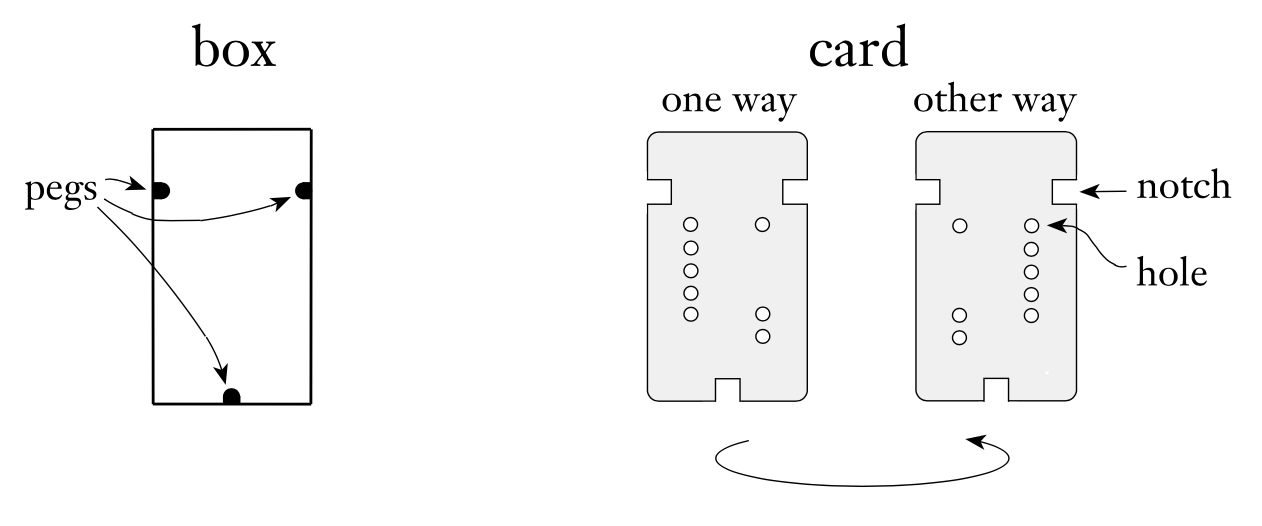
\includegraphics[width=0.75\textwidth]{cards}
  \end{center}
\end{problem}

\end{document}
